\boxde
\BTTN
\Opensolutionfile{ans}[ans/2D1-3-DEON-1]
\begin{ex}%[Dự án tex hóa đề cương Mariecurie - Biên soạn Thầy Nguyễn Ngọc Nguyên]%[2D1B3-2]
    Cho hàm số $y=f(x)$ liên tục trên $\mathbb{R}$ và có bảng biến thiên như hình bên.
    \begin{center}
        
\begin{tikzpicture}
            \tkzTabInit[espcl=3]
            {$x$ /.5, $y'$ /.5,$y$ /1.5}
            {$-\infty$,$0$,$1$,$+\infty$}
            \tkzTabLine{,+,d ,-,$0$,+}
            \tkzTabVar{ -/$-3$,+/$5$,-/$-1$,+/$2$}
        \end{tikzpicture}
    \end{center}
    Khẳng định nào sau đây là đúng?
    \choice
    {Hàm số có giá trị nhỏ nhất bằng $-3$}
    {Hàm số có giá trị nhỏ nhất bằng $-1$}
    {Hàm số có giá trị lớn nhất bằng $-2$}
    {\True Hàm số có giá trị lớn nhất bằng $5$}
    \loigiai
    {
        Dựa vào bảng biến thiên ta thấy hàm số đạt giá trị lớn nhất bằng $5$ tại $x=0$.
    }
\end{ex}
\begin{ex}%[Võ Thị Thùy Trang - DA1]%[2D1Y3-1]
    Cho hàm số $y=f(x)$ liên tục và có bảng biến thiên trong đoạn $[-1;3]$ như hình. Gọi $M$ là giá trị lớn nhất của hàm số $y=f(x)$ trên đoạn $\left[-1;3\right]$. Tìm mệnh đề đúng?
    \begin{center}
        
\begin{tikzpicture}[scale=.76,>=stealth, font=\footnotesize, line join=round, line cap=round]
            \tkzTabInit[nocadre=false,lgt=1.2,espcl=2.5,deltacl=0.6]
            {$x$ /0.6, $y'$ /0.6, $y$ /2.5}
            {$-1$,$0$,$2$,$3$}
            \tkzTabLine{,+,$0$,-,$0$,+,}
            \tkzTabVar{-/$0$,+/$5$,-/$1$,+/$4$}
        \end{tikzpicture}
    \end{center}
    \choice
    {$M=f(-1)$}
    {$M=f(3)$}
    {$M=f(2)$}
    {\True $M=f(0)$}
    \loigiai{
        $M=\max\limits_{[-1;3]} f(x)=f(0)$.
    }
\end{ex}
\begin{ex}%[THPTQG 2020 câu 36 đề 101]%[2D1B3-1]
    Giá trị nhỏ nhất của của hàm số $f(x)=x^3-24x$ trên đoạn $[2;19]$ bằng
    \choice
    {$32\sqrt{2}$}
    {$-40$}
    {\True $-32\sqrt{2}$}
    {$-45$}
    \loigiai{
        Ta có $f'(x)=3x^2-24;\quad f'(x)=0 \Leftrightarrow \hoac{&x=2\sqrt{2}\in [2;19]\\ &x=-2\sqrt{2} \notin [2;19].}$\\
        $f(2)=-40, f(19)=6043, f(2\sqrt{2})=-32\sqrt{2}$.\\
        Vậy $\min\limits_{[2;19]} f(x)=-32\sqrt{2}$.
    }
\end{ex}
\begin{ex}%[Nguyễn Thế Út - DA1]%[2D1B3-1]
    Giá trị lớn nhất của hàm số $y=f(x)=x^4-4x^2+5$ trên đoạn $[-2;3]$ bằng
    \choice{$5$}{$1$}{$122$}{\True$50$}
    \loigiai{
        Hàm số liên tục trên $[-2;3]$.\\
        Ta có $f'(x)=4x^3-8x, f'(x)=0\Leftrightarrow \hoac{& x=0\in [-2;3] \\ & x=-\sqrt{2}\in [-2;3]\\& x=\sqrt{2}\in[-2;3].}$
        \\
        Mà $f(-2)=5, f(3)=50, f(0)=5, f(\sqrt{2})=1, f(-\sqrt{2})=1$.\\
        Vậy $\max\limits_{x \in [-2;3]} f(x)=50$.
    }
\end{ex}
\begin{ex}%[Nguyễn Thế Út - DA1]%[2D1B3-1]
    Tổng giá trị lớn nhất và giá trị nhỏ nhất của hàm số $f(x)=x^5-x^4-3x^3+9$ trên đoạn $[-2;1]$ bằng
    \choice
    {$9$}
    {$10$}
    {$11$}
    {\True $-5$}
    \loigiai{
        Hàm số liên tục trên $[-2;1]$.\\
        Ta có $f'(x)=5x^4-4x^3-9x^2$. $$f'(x)=0\Leftrightarrow 5x^4-4x^3-9x^2=0 \Leftrightarrow\hoac{& x=0\in [-2;1] \\ & x=-1\in[-2;1]\\& x=\dfrac{9}{5}\notin[-2;1].}$$
        Ta có $f(-2)=-15, f(0)=9, f(-1)=10, f(1)=6$.\\
        Suy ra $\max\limits_{x \in [-2;1]} f(x)=10$ và $ \min\limits_{x \in [-2;1]} f(x)=-15 $.\\
        Vậy tổng giá trị lớn nhất và giá trị nhỏ nhất là $ -5 $.
    }
\end{ex}
\begin{ex}%[Võ Thị Thùy Trang - DA1]%[2D1B3-2]%4
    \immini[thm]{Cho hàm số $y=f(x)$ liên tục trên đoạn $[-1;3]$ và có đồ thị như hình. Gọi $M$ và $m$ lần lượt là giá trị lớn nhất và nhỏ nhất của hàm số đã cho trên đoạn $[-1;3]$. Giá trị của $M-m$ bằng
        \choice
        {$0$}
        {$1$}
        {$4$}
        {\True $5$}
    }
    {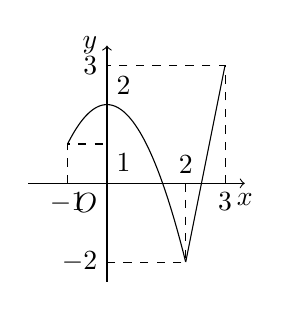
\begin{tikzpicture}[scale=0.5]
            \def\a{-1} \def\b{0} \def\c{2} % Hệ số
            \def\xmin{-2} \def\xmax{3.5}
            \def\ymin{-2.5} \def\ymax{3.5}
            %\draw[color=gray!50,dashed] (\xmin,\ymin) grid (\xmax,\ymax);
            \draw[->] (\xmin,0)--(\xmax,0) node [below]{$x$};
            \draw[->] (0,\ymin)--(0,\ymax) node [left]{$y$};
            \node at (0,0) [below left]{$O$};
            \node at (0,2) [above right]{$2$};
            \draw (2,-2)--(3,3);
            \draw[dashed] (-1,0) node [below] {$-1$}--(-1,1)--(0,1) node [below right] {$1$};
            \draw[dashed] (3,0) node [below] {$3$}--(3,3)--(0,3) node [left] {$3$};
            \draw[dashed] (2,0) node [above] {$2$}--(2,-2)--(0,-2) node [left] {$-2$};
            \clip (\xmin+0.1,\ymin+0.1) rectangle (\xmax-0.5,\ymax-0.1);
            \draw[smooth,samples=300][domain=-1:2] plot(\x,{\a*(\x)^2+\b*(\x)+\c});
    \end{tikzpicture}}
    \loigiai{
        Ta có $M=\max\limits_{[-1;3]} f(x)=f(3)=3$; $m=\min\limits_{[-1;3]} f(x)=f(2)=-2$.\\
        nên $M-m=3-(-2)=5$.
    }
\end{ex}
\begin{ex}%[Dự án tex hóa đề cương Mariecurie - Biên soạn Thầy Nguyễn Ngọc Nguyên]%[2D1K3-1]
    \immini[thm]{Cho hàm số $f(x)$ liên tục trên đoạn $[-2;4]$ và có đồ thị như hình vẽ. Gọi $M,m$ lần lượt là giá trị lớn nhất, nhỏ nhất của hàm số $y=f(|x|)$ trên đoạn $[-2;4]$. Giá trị của $M-m$ bằng
        \choice
        {$4$}
        {\True $3$}
        {$5$}
        {$6$}
    }
    {
        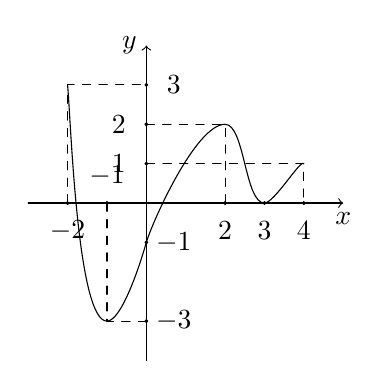
\begin{tikzpicture}[line cap=round, line join=round, scale=0.5]
            \draw[->](-3,0)--(5,0)node[below]{$x$};
            \draw[->](0,-4)--(0,4)node[left]{$y$};
            \draw(-2,3)..controls++(-85:1) and ++(180:0.75)..(-1,-3)..controls++(0:0.35) and++(-106:0.75)..(0,-1)..controls++(74:0.5) and++(180:0.75)..(2,2)..controls ++(0:0.5) and++(180:0.5)..(3,0)..controls++(0:0.25) and++(120:0.15)..(4,1);
            \foreach \x/\y/\m/\g in{0/-3/-3/0,0/3/3/0,-2/0/-2/-90,-1/0/-1/90,0/-1/-1/0,2/0/2/-90,3/0/3/-90,4/0/4/-90,0/1/1/180,0/2/2/180}
            \draw[fill=black](\x,\y)circle(1pt)node[shift={(\g:0.35)}]{$\m$};
            \draw[dashed](-2,0)--(-2,3)--(0,3)(-1,0)--(-1,-3)--(0,-3)(2,0)--(2,2)--(0,2)(0,1)--(4,1)--(4,0);
        \end{tikzpicture}
    }
    \loigiai
    {
        Ta vẽ đồ thị của hàm số $y=f(|x|)$ nhứ sau: Giữa nguyên phần đồ thị nằm bên phải trục $Oy$ của hàm số $y=f(x)$, xóa bỏ phần nằm bên trái. Lấy đối xứng phần đồ thị nằm bên phải qua trục Oy.\\
        Từ đó ta có giá trị lớn nhất và nhỏ nhất của hàm số $y=f(|x|)$ trên $[-2;4]$ lần lượt là $M=2$ và $m=-1$.\\ Suy ra $M-m=3$.
    }
\end{ex}
\begin{ex}%[Nguyễn Thế Út - DA1]%[2D1B3-1]
    Giá trị lớn nhất của hàm số $f(x)=\dfrac{x-m^2}{x+1}$ trên đoạn $[0;1]$ bằng.
    \choice
    {$\dfrac{1+m^2}{2}$}
    {$-m^2$}
    {\True $\dfrac{1-m^2}{2}$}
    {$-\dfrac{m^2-1}{2}$}
    \loigiai{
        \begin{itemize}
            \item Tập xác định $\mathscr{D}=\mathbb{R}\setminus\{-1\}$.
            \item Ta có $f'(x)=\dfrac{1+m^2}{(x+1)^2}>0$, $\forall x\in\mathscr{D}$.
            \item Do đó hàm số đồng biến trên $[0;1]$. Suy ra $\max\limits_{[0;1]}f(x)=f(1)=\dfrac{1-m^2}{2}$.
        \end{itemize}
    }
\end{ex}
\begin{ex}%[Nguyễn Thế Út - DA1]%[2D1B3-1]
    Giá trị nhỏ nhất của hàm số $f(x)=\dfrac{2x-1}{3x-6}$ trên đoạn $[0;3]$ là
    \choice
    {$\dfrac{1}{6}$}
    {$\dfrac{5}{3}$}
    {$\dfrac{1}{2}$}
    {\True không tồn tại}
    \loigiai{
        \begin{itemize}
            \item Tập xác định $\mathscr{D}=\mathbb{R}\setminus\{2\}$.
            \item Ta có $f'(x)=-\dfrac{9}{(3x-6)^2}<0$, $\forall x\in\mathscr{D}$.
            Bảng biến thiên
            \begin{center}
                
\begin{tikzpicture}[>=stealth,scale=1]
                    \tkzTabInit[lgt=1.2,espcl=3]
                    {$x$/0.7,$f’(x)$/0.7,$f(x)$/2.5}
                    {$0$,$2$,$3$}
                    \tkzTabLine{ ,-,d,-,}
                    \tkzTabVar{+/$\dfrac{1}{6}$,-D+/$-\infty$/$+\infty$,-/$\dfrac{5}{3}$}
                \end{tikzpicture}
            \end{center}
            \item Do đó hàm số không có giá trị nhỏ nhất trên $[0;3]$.
        \end{itemize}
    }
\end{ex}
\begin{ex}%[Nguyễn Thế Út - DA1]%[2D1B3-1]
    Giá trị nhỏ nhất của hàm số $y=x+\dfrac{9}{x}$ trên đoạn $[2;4]$ bằng
    \choice
    {$\dfrac{13}{2}$}
    {\True $6$}
    {$\dfrac{11}{2}$}
    {$\dfrac{25}{4}$}
    \loigiai{
        Ta có $y'=1-\dfrac{9}{x^2}$.
        $$y'=0\Leftrightarrow \hoac{&x=3\in [2;4]\\&x=-3\notin[2;4].}$$
        Khi đó $f(2)=\dfrac{13}{2}$, $f(3)=6$, $f(4)=\dfrac{25}{4}$, suy ra $\min\limits_{[2;4]}f(x)=6$.
    }
\end{ex}
\begin{ex}%[Nguyễn Trần Phong, Dự án 6 đề cương HKI k12 Marie]%[2D1B3-1]
    Tập giá trị của hàm số $f(x)= \sin^3 x -2 \sin^2 x+ 5$ là
    \choice
    {$[0;1] $}
    {\True $ [2;5]$}
    {$ [-1;1]$}
    {$[2;4] $}
    \loigiai{
        Đặt $t= \sin x$, $t \in [-1;1]$. Khi đó ta được $g(t)= t^3 -2t^2 +5$ với $t \in [-1;1]$.\\
        $g'(t) = 3t^3 -4t.$\\
        Cho $g'(t) =0 \Leftrightarrow \hoac{& t=0 \in [-1;1]\\& t= \pm \dfrac{2\sqrt{3}}{3} \notin [-1;1].}$\\
        Xét $g(-1)=2$; $g(0) =5$; $g(1)= 4$.\\
        Suy ra với $t \in [-1;1]$ thì $2 \le g(t) \le 5 $. Do đó tập giá trị của hàm $f$ là $[2;5]$.
    }
\end{ex}
\begin{ex}%[Nguyễn Trần Phong, Dự án 6 đề cương HKI k12 Marie]%[2D1B3-1]
    Tổng giá trị lớn nhất và nhỏ nhất của hàm số $f(x)=\sin^4 x - \cos^2 x$ bằng
    \choice
    {$- \dfrac{1}{4} $}
    {$- \dfrac{9}{4} $}
    {\True $0 $}
    {$-\dfrac{5}{4} $}
    \loigiai{
        Ta có $f(x) = (1-\cos^2 x)^2 - \cos^2 x$.\\
        Đặt $t= \cos^2 x$, $t \in [0;1]$. Khi đó ta có $g(t) = (1-t)^2 - t= t^2 - 3t +1$.\\
        $g'(t) = 2t-3 <0 $ với mọi $t \in [0;1]$. \\
        Suy ra $\displaystyle \min_{[0;1]} g(t) = g(1)= -1$ và $\displaystyle \max_{[0;1]} g(t) = g(0)= 1$.\\
        Vậy tổng giá trị lớn nhất và nhỏ nhất của hàm $f$ là $1 + (-1) =0.$}
\end{ex}
\begin{ex}%[2D1K3-1]%[Dự án TEX hóa đề cương Marie Curie - Ân Trương]
    Cho hàm số $ f(x)=\dfrac{mx+1}{x-m} $ ($ m $ là tham số thực) thỏa mãn $ \max\limits_{[1 ; 2]} f(x)=-2 $. Khi đó giá trị $ m $ bằng
    \choice
    {$4$}
    {\True$3$}
    {$2$}
    {$1$}
    \loigiai{
        Tập xác định $ \mathscr{D} = \mathbb{R} \setminus\{m\}$.\\
        Để hàm số có giá trị lớn nhất trên $ [1;2] $ thì $ m\notin [1;2] $.\\
        Ta có $ f'(x)=\dfrac{-m^2-1}{(x-m)^{2}} <0, \forall x \ne m$.\\
        $ \Rightarrow \max\limits_{[1 ; 2]}f(x)=f(1)=\dfrac{m+1}{1-m} $.\\
        Theo đề bài
        \begin{eqnarray*}
            &&\max\limits_{[1 ; 2]}f(x)=-2\\
            &\Leftrightarrow& \dfrac{m+1}{1-m}=-2\\
            &\Leftrightarrow& m+1=2m-2\\
            &\Leftrightarrow& m=3.
        \end{eqnarray*}
    }
\end{ex}
\begin{ex}%[Nguyễn Trần Phong, Dự án 6 đề cương HKI k12 Marie]%[2D1K3-1]
    Với giá trị nào của $m$ để giá trị lớn nhất của hàm số $f(x)= - x^3 -3x^2 +m$ trên $[-1;1]$ bằng $0$?
    \choice
    {$ 0$}
    {$4 $}
    {\True $2 $}
    {$6 $}
    \loigiai{
        Ta có $f'(x)= -3x^2 -6x$.\\
        Cho $f'(x)=0 \Leftrightarrow \hoac{& x=0 \in [-1;1]\\& x= -2 \notin [-1;1].}$\\
        Xét $f(-1)= -2 + m $; $f(1)= -4 + m$.\\
        Suy ra $\displaystyle \max_{[-1;1]} f(x) = -2 + m$.\\
        Theo đề bài, $-2+ m=0 \Leftrightarrow m=2.$}
\end{ex}
\begin{ex}%[KSCL T12, Chu Văn An, Hà Nội, 2018-Cau21]%[2D1K3-6]%
    Một chất điểm chuyển động theo quy luật $s(t)=t^2-\dfrac{1}{6}t^3$ (m). Tìm thời điểm $t$ (giây) mà tại đó vận tốc $v$ (m/s) của chuyển động đạt giá trị lớn nhất.
    \choice
    {\True $t=2$}
    {$t=0{,}5$}
    {$t=2{,}5$}
    {$t=1$}
    \loigiai{
        Ta có $v(t)=s'(t)=2t-\dfrac{1}{2}t^2$. Suy ra $v'(t)=2-t$ và $v'(t)=0\Leftrightarrow t=2$.\\
        Bảng biến thiên
        \begin{center}
            
\begin{tikzpicture}[>=stealth]
                \tkzTabInit[nocadre,lgt=1.2,espcl=2]
                {$t$ /0.8, $v'(t)$ /0.8, $v(t)$ /2}
                {$ $, $2$, $ $}
                \tkzTabLine{ , +, 0, -, }
                \tkzTabVar{-/, +/ $2$, -/}
            \end{tikzpicture}
        \end{center}
        Vậy chất điểm đạt vận tốc lớn nhất tại thời điểm $t=2$ (giây).
    }
\end{ex}
\begin{ex}%[Thi Thử L1, Trần Phú, Hà Tĩnh]%[2D1K3-6]%[Trần Phong, 12EX-8]%
    \immini[thm]{
        Từ một tấm tôn có hình dạng là nửa hình tròn bán kính $R=3$, người ta muốn cắt ra một hình chữ nhật (hình vẽ bên). Diện tích lớn nhất có thể của tấm tôn hình chữ nhật là
        \choice
        {$\dfrac{9}{2}$}
        {$6\sqrt2$}
        {\True $9$}
        {$9\sqrt2$}
    }
    {
        \begin{tikzpicture}[thick,scale=0.7]
            \draw [-] (-4,0)--(4,0);
            \draw [-] (-3,0)--(-2.99,2.65)--(2.99,2.65)--(3,0);
            \draw[smooth,samples=200,variable=\t,domain=0:180] plot({(4)*cos (\t)},{(4)*sin(\t)});
            \draw (0,0) [fill=black] circle (1pt) node[below]{$O$};
            \draw (-3,0) [fill=black] circle (1pt) node[below]{$Q$};
            \draw (3,0) [fill=black] circle (1pt) node[below]{$P$};
            \draw (-2.99,2.65) [fill=black] circle (1pt) node[left]{$M$};
            \draw (2.99,2.65) [fill=black] circle (1pt) node[right]{$N$};
            \draw[pattern=north east lines,pattern color=black!50!] (-3,0)--(-2.99,2.65)--(2.99,2.65)--(3,0);
        \end{tikzpicture}
    }
    \loigiai{
        Đặt $OQ=x,\ (0<x<3) \Rightarrow MQ=\sqrt{MO^2-OQ^2}=\sqrt{9-x^2}$.\\
        Ta có $S_{MNPQ}=PQ\cdot MQ=2x\cdot\sqrt{9-x^2}\le 2\cdot\dfrac{x^2+9-x^2}{2}=9.$\\
        Dấu $``=$ xảy ra khi $x=\dfrac{3\sqrt2}{2}.$
    }
\end{ex}
\begin{ex}%[Đề kiểm tra HK1 THPT Lương Ngọc Quyến - Thái Nguyên, 2020-2021]%[Lý Văn Hoàng, 12-EX-5-2021]%[2D1K3-6]%
    Người ta xây một bể chứa nước với hình dạng khối hộp chữ nhật không nắp có thể tích bằng $\dfrac{500}{3}$ m$^3$. Đáy bể là hình chữ nhật có chiều dài gấp đôi chiều rộng. Giá thuê nhân công để xây bể là $600{,}000$ đồng/m$^2$. Hãy tính chi phí thuê nhân công thấp nhất để xây dựng bể nước.
    \choice
    {$75$ triệu đồng}
    {$86$ triệu đồng}
    {\True $90$ triệu đồng}
    {$85$ triệu đồng}
    \loigiai{
        \immini[thm]{Gọi chiều rộng của đáy là $x$ (m) $(x>0)$ thì chiều dài của bể là $2x$ (m).\\
            Gọi chiều cao của bể nước là $h$ (m) $(h>0)$.\\
            Ta có $V=h\cdot x \cdot 2x=\dfrac{500}{3} \Leftrightarrow h=\dfrac{250}{3x^2}$.\\
            Vì bể này không có nắp nên diện tích xung quanh của bể sẽ bằng tổng diện tích bốn mặt bên cộng với diện tích một mặt đáy nên ta có $S= 2\cdot (2xh+xh)+ 2x^2$ $(^*)$.\\
            Thay $h= \dfrac{250}{3x^2}$ vào $(^*)$ ta được $S= \dfrac{500}{x} +2x^2$.\\
            Xét hàm $f(x) = \dfrac{500}{x} +2x^2, \, \forall x>0$.\\
            Ta có $f'(x) =-\dfrac{500}{x^2} +4x \Leftrightarrow f'(x)=0 \Leftrightarrow 4x^3=500 \Leftrightarrow x=5$.\\
        }
        {\begin{tikzpicture}[scale=1, font=\footnotesize, line join=round, line cap=round, >=stealth]
                \def\bc{3} % cạnh BC
                \def\ba{1.5} % cạnh BA
                \def\h{2} % đường cao
                \def\gocB{35} % góc B của đáy
                \coordinate (B) at (0,0);
                \coordinate (A) at (\gocB:\ba);
                \coordinate (C) at (\bc,0);
                \coordinate (D) at ($(C)-(B)+(A)$);
                \coordinate (A') at ($(A)+(90:\h)$);
                \coordinate (B') at ($(B)-(A)+(A')$);
                \coordinate (C') at ($(C)-(A)+(A')$);
                \coordinate (D') at ($(D)-(A)+(A')$);
                \draw (B')--(B)--(C)--(D)--(D')--(A')--(B')--(C')--(D') (C)--(C');
                \tkzInterLL(A,A')(B',C') \tkzGetPoint{M}
                \draw (A')--(M);
                \draw[dashed] (M)--(A)--(D) (A)--(B);
                \tkzLabelSegment[right](B,B'){$h$}
                \tkzLabelSegment[below](B,C){$2x$}
                \tkzLabelSegment[right](D,C){$x$}
        \end{tikzpicture}}
        Bảng biến thiên
        \begin{center}
            
\begin{tikzpicture}[scale=1, font=\footnotesize, line join=round, line cap=round, >=stealth]
                \tkzTabInit[nocadre=false,lgt=1,espcl=2,deltacl=0.5]{$x$/.7 ,$y'$/.7,$y$/2}
                {$0$ , $5$ , $+\infty$}
                \tkzTabLine{ , - , $0$ , + , }
                \tkzTabVar{+/$+\infty$ , -/$150$ , +/$+\infty$}
            \end{tikzpicture}
        \end{center}
        Dựa vào bảng biến thiên ta thấy $\min S= 150 \Leftrightarrow x=5$ và giá tiền thuê nhân công là $ 90$ triệu đồng.
    }
\end{ex}
\begin{ex}%[2D1K3-1]%[Dự án TEX hóa đề cương Marie Curie - Ân Trương]
    \immini[thm]
    {
        Cho hàm số $ y=f(x) $ có đạo hàm liên tục trên $ \mathbb{R} $ và đồ thị hàm số $ y=f'(x) $ như hình vẽ. Biết rằng $ f(0)+f(1)-2f(2)=f(4)-f(3)$. Khi đó giá trị nhỏ nhất và giá trị lớn nhất của hàm số trên $ [0;4] $ lần lượt là
        \choice
        {\True$f(4)$ và $ f(2)$}
        {$f(4)$ và $ f(1)$}
        {$f(0)$ và $ f(2)$}
        {$f(1)$ và $ f(2)$}
    }
    {
        \begin{tikzpicture}[>=stealth,x=1cm,y=1cm,scale=0.9,font=\footnotesize]
            \path
            (-0.2,-0.9) coordinate (P)
            (0,0) coordinate (O)
            (5,0) coordinate (Bf)(-1,0) coordinate (Af)
            (0,0) coordinate (O)node[above left]{$ O $}
            (0.5,1.3) coordinate (M1)
            (2.1,-1.1) coordinate (Q)
            (4,0.8) coordinate (M2)node[shift={(-0.7,0.2)}]{$ y=f'(x)$}
            ;
            %\draw[red] (O)--(M1)--(Q)--(M2);
            \draw[name path=ox] (Af)--(Bf);
            \draw[name path=fx,thick,black]
            (P)..controls +(70:0.25) and+(-175:0.35)..
            (M1)..controls +(-5:0.35) and+(175:0.5)..(Q)
            ..controls +(10:0.5) and+(-110:0.25)..(M2)
            ;
            \path[name intersections={of=fx and ox, by={O,B1,B2}}]
            (B1)node[above]{$ 2 $};
            \path ($(B1)!2/3!(B2)$) coordinate (B3)node[above]{$ 4 $}
            ($(B3)+(0,-0.7)$) coordinate (P1);
            \draw[dashed](B3)--(P1);
            %Vẽ hệ trục tọa dộ:
            \draw[->] (-1.2,0)--(0,0)--(5,0) node[below]{$x$};
            \draw[->] (0,-1.5) --(0,2.5) node[left]{$y$};
            %	Node các điểm
            \foreach \p in {O,B1,B2,P1}
            \fill (\p) circle (1.5pt) ;
        \end{tikzpicture}
    }
    \loigiai{
        Ta có bảng biến thiên của hàm số y=f(x)
        \begin{center}
            
\begin{tikzpicture}
                \tkzTabInit[nocadre=false,lgt=1.2,espcl=2.5,deltacl=0.6]
                {$x$ /0.6,$f’(x)$ /0.6,$f(x)$ /2}
                {$0$,$1$,$2$,$3$,$4$}
                \tkzTabLine{,,+,,0,,-,,}
                \tkzTabVar{-/$f(0)$,R/,+/$2$,R/,-/$f(4)$}
                \tkzTabIma{1}{3}{2}{$ f(1) $}
                \tkzTabIma{3}{5}{4}{$ f(3) $}
            \end{tikzpicture}
        \end{center}
        Từ bảng biến thiên của hàm số $ y=f(x) $ trên đoạn $ [0;4] $ ta thấy $ \max\limits_{[0;4]}f(x)=f(2) $.\\
        Ta có
        \begin{eqnarray*}
            &&f(0)+f(1)-2f(2)=f(4)-f(3)\\
            &\Leftrightarrow& f(1)+f(3)-2 f(2)=f(4)-f(0)\\
            &\Leftrightarrow& f(1)-f(2)+f(3)-f(2)=f(4)-f(0)\quad (\ast)\\
            &\xrightarrow[f(1)-f(2)<0]{f(3)-f(2)<0}&f(1)-f(2)+f(3)-f(2)<0.
        \end{eqnarray*}
        Từ $ (\ast) \Rightarrow f(4)-f(0)<0 \Leftrightarrow f(4)<f(0) \Rightarrow \min\limits_{[0;4]}f(x)=f(4) $.\\
        Do đó $ \min\limits_{[0;4]}f(x)=f(4), \quad \max\limits_{[0;4]}f(x)=f(2). $.
    }
\end{ex}
\begin{ex}%[Phạm Đình Quang-DA1]%[2D1K1-4]
    \immini[thm]
    {
        Cho hàm số $y=f(x)$ liên tục trên $[-5;3]$, có đồ thị như hình vẽ. Tìm $m$ để bất phương trình $f\left(\sqrt{4x-x^2}\right)\geq m$ có nghiệm $x\in [0;4]$
        \choice
        {$m\leq 3$}
        {$m\leq 0$}
        {\True $m\leq 4$}
        {$m\leq -1$}
    }
    {
        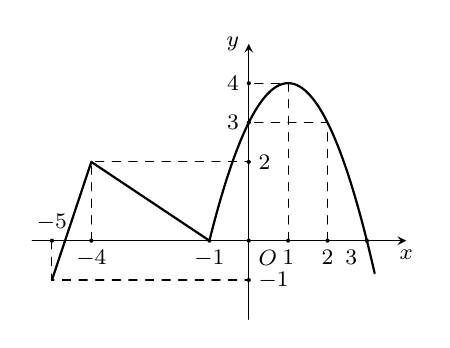
\begin{tikzpicture}[>=stealth,line join=round,line cap=round,font=\footnotesize,scale=0.5]
            \draw[->] (-5.5,0)--(4,0) node[below]{$x$};
            \draw[->] (0,-2)--(0,5) node[left]{$y$};
            \fill[name=O] (0,0) circle (1.5pt) node[below right] {$O$};
            \draw[thick] (-5,-1)--(-4,2)--(-1,0);
            \draw[thick, smooth, samples=300, domain= -1:3.2] plot(\x,{-(\x)^2+2*(\x)+3}) node[left]{$ $};
            \draw[dashed] (-5,0)|-(0,-1)
            (-4,0)|-(0,2)
            (1,0)|-(0,4)
            (2,0)|-(0,3);
            \foreach \x/\p in {-5/90,-4/-90,-1/-90,1/-90,2/-90,3/-100}
            \fill (\x,0) circle (1.5pt)coordinate[label=\p:$\x$];
            \foreach \y/\p in {-1/0,2/0,3/180,4/180}
            \fill (0,\y) circle (1.5pt)coordinate[label=\p:$\y$];
        \end{tikzpicture}
    }
    \loigiai{
        Đặt $\sqrt{4x-x^2}=t$, $x\in [0;4]\Rightarrow t\in [0;2]$.\\
        Bất phương trình bài cho trở thành $f(t)\geq m$\hfill (1).\\
        Để bất phương trình $f(\sqrt{4x-x^2})\geq m$ có nghiệm thì bất phương trình $(1)$ phải có nghiệm.\\
        Với $t\in [0;2]$ suy ra $f(t)\in [3;4]$.\\
        Vậy $(1)$ có nghiệm khi $m\leq 4$.
    }
\end{ex}
\begin{ex}%Ví dụ 9%[Phat Dang Tan - DA1]%[2D1B5-4]
    Cho hàm số $y=f(x)$ liên tục trên $\mathbb{R}$ và có đồ thị như hình vẽ. Có bao nhiêu giá trị nguyên của $m$ để phương trình $f\left(f\left(\sin x\right)\right)=m$ có nghiệm thuộc khoảng $\left(0;\pi\right)$?
    \begin{center}
        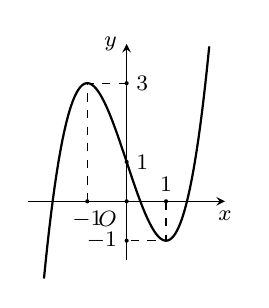
\begin{tikzpicture}[font=\footnotesize,>=stealth,x=1cm,y=1cm,scale=0.5]
            \draw[->] (-2.5,0)--(2.5,0) node [below]{$x$};
            \draw[->] (0,-1.5)--(0,4) node [left]{$y$};
            \draw[samples=300,thick,domain=-2.1:2.1]plot(\x,{(\x)^3-3*(\x)+1});
            \draw[dashed](1,0)--(1,-1)--(0,-1) (-1,0)--(-1,3)--(0,3);
            \fill[black] (1,0)node[above]{$1$} circle (1.5pt) (-1,0)node[below]{$-1$} circle (1.5pt) (0,0)node[below left]{$O$} circle (1.5pt) (0,1)node[right]{$1$} circle (1.5pt) (0,3)node[right]{$3$} circle (1.5pt) (0,-1)node[left]{$-1$} circle (1.5pt);
        \end{tikzpicture}
    \end{center}
    \choice
    {$1$}
    {$2$}
    {$3$}
    {\True $4$}
    \loigiai{
        Đặt $t=\sin x$. Khi đó với $x\in \left(0;\pi\right)$ thì $\sin x\in (0;1]$.\\
        Dựa vào đồ thị $f(x)$ suy ra $a=f(t)\in [-1;1)\Rightarrow f(a)\in (-1;3]$.\\
        Suy ra phương trình $f(a)=m$ có nghiệm $x\in (0;\pi)$ khi và chỉ khi $m\in(-1;3]$.\\
        Mà $m$ nhận giá trị nguyên nên $m\in\left\{0,1,2,3\right\}$.\\
        Vậy có $4$ giá trị nguyên của $m$ thỏa yêu cầu.
    }
\end{ex}
\BTTF
\begin{ex}%[2D1N3-2]%[Dự án EX-TF-TLN-2024 - Đợt 1]%[Thành Đức Trung]
    \immini[thm]
    {
        Cho hàm số $y=f(x)$ có đồ thị như hình vẽ.
        \choiceTF
        {Hàm số đồng biến trên khoảng $(-\infty;1)$}
        {Giá trị cực tiểu của hàm số bằng $1$}
        {\True $\min\limits_{(-2;1)} f(x)=0$}
        {$\max\limits_{\mathbb{R}} f(x)=4$}
    }
    {
        \begin{tikzpicture}[line join = round, line cap = round,>=stealth,font=\footnotesize,scale=0.7]
            \def\xt{-3} \def\xp{3} \def\yd{-1} \def\yt{5}
            \def\a{-1}
            \def\b{0}
            \def\c{3}
            \def\d{2}
            \draw[->] (\xt,0)--(\xp,0) node[below]{$x$};
            \draw[->] (0,\yd)--(0,\yt) node[left]{$y$};
            \foreach \x/\y/\z/\g in
            {
                0/0/O/-135, -2/0/-2/-90, -1/0/-1/-90, 1/0/1/-90, 0/2/2/135, 0/4/4/135
            }
            \draw[fill=black] (\x,\y) circle(1pt) coordinate (\z) ($(\z)+(\g:3.5mm)$) node{$\z$};
            \draw[dashed] (-2,0)--(-2,4)--(1,4)--(1,0);
            \begin{scope}
                \clip (\xt+0.1,\yd+0.1) rectangle (\xp-0.1,\yt-0.1);
                \draw[samples=150,smooth,domain=\xt:\xp] plot(\x,{\a*(\x)^3+(\b)*(\x)^2+(\c)*\x+(\d)});
            \end{scope}
        \end{tikzpicture}
    }
    \loigiai{
        Nhìn vào đồ thị ta thấy
        \begin{itemchoice}
            \itemch \textbf{Đúng}.
            \itemch \textbf{Sai}. Vì giá trị cực tiểu của hàm số là $0$.
            \itemch \textbf{Đúng}.
            \itemch \textbf{Sai}. Vì $\lim\limits_{x\to -\infty} = +\infty$ nên không tồn tại $\max\limits_{\mathbb{R}} f(x)$.
        \end{itemchoice}
    }
\end{ex}
\begin{ex}%[2D1N3-2]%[Dự án EX-TF-TLN-2024 - Đợt 1]%[Thành Đức Trung]
    Khảo sát hàm số $f(x)=3x+1+\dfrac{3}{x+1}$ trên khoảng $(-4;2)$.
    \choiceTF
    {\True Giá trị lớn nhất của $f(x)$ trên $(-4;-1)$ bằng $-8$}
    {\True Hàm số $f(x)$ có hai điểm cực trị trên $(-4;2)$}
    {\True Giá trị nhỏ nhất của $f(x)$ trên $(-1;2)$ bằng $4$}
    {\True Không tồn tại giá trị lớn nhất của $f(x)$ trên $(-4;2)$}
    \loigiai{
        Xét hàm số $f(x)=3x+1+\dfrac{3}{x+1}$ trên khoảng $(-3;1)$. \\
        Ta có
        \begin{itemize}
            \item tập xác định $\mathscr{D} = \mathbb{R}\setminus \{-1\}$ nên $\mathscr{D} \cap (-4;2) = (-4;-1)\cup (-1;2)$.
            \item $f'(x) = 3 - \dfrac{3}{(x+1)^2}$ nên $f'(x) = 0 \Leftrightarrow \hoac{&x=0\\ &x=-2.}$
        \end{itemize}
        Khi đó ta có bảng biến thiên
        \begin{center}
            
\begin{tikzpicture}[scale=1,font=\footnotesize, line join=round, line cap=round, >=stealth, transform shape]
                \tkzTabInit[nocadre=false,lgt=1.2,espcl=2.5,deltacl=0.6]
                {$x$ /0.6, $f'(x)$ /0.6, $f(x)$ /2}
                {$-4$,$-2$,$-1$,$0$,$2$}
                \tkzTabLine{,+,z,-,d,-,z,+,}
                \tkzTabVar{-/$-12$,+/$-8$,-D+/$-\infty$ /$+\infty$,-/$4$,+/$8$}
            \end{tikzpicture}
        \end{center}
        Nhìn vào bảng biến thiên ta thấy
        \begin{itemchoice}
            \itemch \textbf{Đúng}.
            \itemch \textbf{Đúng}. Vì hai điểm cực trị là $x=-2$ và $x=0$.
            \itemch \textbf{Đúng}.
            \itemch \textbf{Đúng}. Vì $\lim\limits_{x\to -1^+} y = +\infty$ nên không tồn tại $\max\limits_{(-4;2)} f(x)$.
        \end{itemchoice}
    }
\end{ex}
\begin{ex}%[2D1N3-2]%[Dự án EX-TF-TLN-2024 - Đợt 1]%[Thành Đức Trung]
    Cho hàm số $y=f(x)$ là hàm liên tục trên $\mathbb{R}$ và có bảng biến thiên như hình vẽ.
    \begin{center}
        
\begin{tikzpicture}[scale=1,font=\footnotesize, line join=round, line cap=round, >=stealth, transform shape]
            \tkzTabInit[nocadre = false,lgt=1.5,espcl=2]
            {$x$/1,$y'$/1,$y$/2}
            {$-\infty$,$-1$,$0$,$1$,$+\infty$}
            \tkzTabLine{,+,z,-,z,+,z,-,}
            \tkzTabVar{-/$-\infty$ , +/$4$,-/$3$, +/$4$,-/$-\infty$}
        \end{tikzpicture}
    \end{center}
    \choiceTF
    {$\min\limits_{\mathbb{R}} y = 3$}
    {\True $\max\limits_{\mathbb{R}} y = 4$}
    {\True Giá trị cực tiểu của hàm số là $3$}
    {Hàm số có $3$ điểm cực đại}
    \loigiai{
        Nhìn vào bảng biến thiên ta thấy
        \begin{itemchoice}
            \itemch \textbf{Sai}. Vì $\lim\limits_{x\to -\infty} y = -\infty$ nên không tồn tại $\min\limits_{\mathbb{R}} f(x)$.
            \itemch \textbf{Đúng}.
            \itemch \textbf{Đúng}.
            \itemch \textbf{Sai}. Vì hàm số chỉ có $2$ điểm cực đại.
        \end{itemchoice}
    }
\end{ex}
\begin{ex}%[2D1N3-2]%[Dự án EX-TF-TLN-2024 - Đợt 1]%[Thành Đức Trung]
    \immini[thm]
    {
        Cho hàm số $y=f(x)$ xác định trên $\mathbb{R}\setminus{\{2\}}$, liên tục trên mỗi khoảng xác định và có bảng biến thiên như hình vẽ.
    }
    {
        
\begin{tikzpicture}[scale=0.8,font=\footnotesize, line join=round, line cap=round, >=stealth, transform shape]
            \tkzTabInit[lgt=1.2, espcl=3]
            {$x$/1,$y'$/1,$y$/2.5}
            {$-\infty$,$0$,$2$,$+\infty$}
            \tkzTabLine{ ,+,$0$,-,d,+, }
            \tkzTabVar{-/$0$,+/$3$,-D-/$-3$ /$-3$,+/$10$}
        \end{tikzpicture}
    }
    \choiceTF
    {Giá trị lớn nhất của hàn số trên $\mathbb{R}\backslash{\{2\}}$ bằng $10$}
    {Giá trị cực đại của hàm số là $y_\text{CĐ}=10$}
    {Giá trị cực tiểu của hàm số là $y_\text{CT}=-3$}
    {Giá trị nhỏ nhất của hàm số trên $\mathbb{R}\backslash{\{2\}}$ là $-3$}
    \loigiai{
        Nhìn vào bảng biến thiên ta thấy
        \begin{itemchoice}
            \itemch \textbf{Sai}. Vì $\lim\limits_{x\to +\infty} y = 10$ nên không đảm bảo tồn tại $x$ để $f(x) = 10$.
            \itemch \textbf{Sai}. Vì $y_\text{CĐ} = 3$
            \itemch \textbf{Sai}. Vì hàm số không có cực tiểu.
            \itemch \textbf{Sai}. Vì $\lim\limits_{x\to 2^+} y = \lim\limits_{x\to 2^-} y = 3$ nên không tồn tại $x$ để $f(x) = -3$.
        \end{itemchoice}
    }
\end{ex}
\BTTL
\begin{ex}
    Tìm giá trị lớn nhất và giá trị nhỏ nhất của hàm số có đồ thị được cho ở hình sau
    \begin{center}
        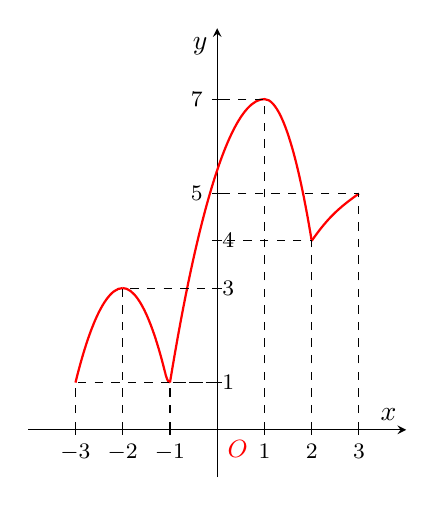
\begin{tikzpicture}[>=stealth,scale=0.6]
            %	\draw[line width=0.1pt,dashed] (0,0) grid (6,6);
            \draw[-> ] (-4,0) -- (4,0)node[above left] {$x$};
            \draw[-> ] (0,-1) -- (0,8.5)node[below left] {$y$};
            \draw [thick,red](0,0) node[below right] {\small $O$};
            \draw [thick,red] (-3,1) parabola [bend at end] (-2,3) ;
            \draw[thick,red] (-2,3) parabola (-1.1,1.2);
            \draw [thick,red](-1.1,1.2) parabola[bend at end] (-1,1);
            \draw[thick,red] (-1,1) parabola bend (1,7) (2,4);
            \draw[thick,red] (2,4) to[bend left=10] (3,5);
            \foreach \x in {1,2,3,-3,-2,-1}\draw (\x,0.1)--(\x,-0.1) node [below] {\footnotesize $\x$};
            \foreach \y in {1,3,4}\draw (0.1,\y)--(-0.1,\y) node [right] {\footnotesize $\y$};
            \foreach \y in {5,7}\draw (0.1,\y)--(-0.1,\y) node [left] {\footnotesize $\y$};
            \draw[dashed] (-3,0) -- (-3,1) -- (0,1);
            \draw[dashed] (-2,0) -- (-2,3)--(0,3);
            \draw[dashed] (-1,0) -- (-1,1) -- (0,1);
            \draw[dashed] (2,0) -- (2,4) -- (0,4);
            \draw[dashed] (3,0) -- (3,5) -- (0,5);
            \draw[dashed] (1,0) -- (1,7) -- (0,7);
        \end{tikzpicture}
    \end{center}
    \shortans{$M=7$, $=1$}
\end{ex}
\begin{ex}%[2D1V3-2]%[Dự án EX-TF-TLN-2024 - Đợt 1]%[Thành Đức Trung]
    Cho $a$, $b$ là các số thực thỏa mãn $0<a<1<b$, $ab>1$. Tìm giá trị lớn nhất của biểu thức $P=\log_a ab+\dfrac{4}{\left(1-\log_ab\right)\cdot \log_{\frac{a}{b}}ab}$.
    \shortans{$-4$}
    \loigiai{
        Ta có $P=1+\log_ab+\dfrac{4}{1+\log_ab}$.\\
        Do $0<a<1<b$ và $ab>1$ nên suy ra $\log_ab = \log_ab + 1 - 1 = \log_a(ab) - 1 < \log_a 1 - 1 < -1$.\\
        Xét hàm số $f(t)=1+t+\dfrac{4}{1+t}$ trên $(-\infty;-1)$ có $f'(t) = 1 - \dfrac{4}{(t+1)^2}$ nên
        \[
        f'(t) = 0 \Leftrightarrow (t+1)^2 = 4 \Leftrightarrow \hoac{&t=1 & &\text{ (loại)}\\ &t = -3 & &\text{ (thoả mãn).}}
        \]
        Khi đó ta có bảng biến thiên
        \begin{center}
            
\begin{tikzpicture}[scale=1,font=\footnotesize, line join=round, line cap=round, >=stealth, transform shape]
                \tkzTabInit[nocadre=false,lgt=1.2,espcl=2.5,deltacl=0.6]
                {$t$/0.6,$f'(t)$/0.6,$f(t)$/2}
                {$-\infty$,$-3$,$-1$}
                \tkzTabLine{,+,0,-,}
                \tkzTabVar{-/ $-\infty$, +/$-4$, -/$-\infty$}
            \end{tikzpicture}
        \end{center}
        Vậy $\max P = \max\limits_{(-\infty,-1)} f(t) = -4$.
    }
\end{ex}
\begin{ex}%[2D1H3-2]%[Dự án EX-TF-TLN-2024 - Đợt 1]%[Thành Đức Trung]
    Gọi $ M $, $ m $ lần lượt là giá trị lớn nhất và giá trị nhỏ nhất của hàm số $ y=\dfrac{\sqrt{x^2-1}}{x-2} $ trên tập hợp $ \mathscr{D}=(-\infty;-1)\cup\left[ 1;\dfrac{3}{2} \right] $. Tính giá trị biểu thức $ P=M^2+m^2$.
    \shortans{$5$}
    \loigiai
    {
        Ta có $ y'=\dfrac{1-2x}{(x-2)^2\sqrt{x^2-1}} $, $ y'=0\Leftrightarrow 1-2x=0 \Leftrightarrow x=\dfrac{1}{2}\notin\mathscr{D}$.\\
        Bảng biến thiên
        \begin{center}
            
\begin{tikzpicture}[scale=1,font=\footnotesize, line join=round, line cap=round, >=stealth, transform shape]
                \tkzTabInit[nocadre=false,lgt=1.2,espcl=2.5,deltacl=0.6]
                {$x$/0.6,$y'$/0.6,$y$/1.8}{$-\infty$,$-1$,$1$,$\frac{3}{2}$}
                \tkzTabLine{,+,d, ,d,-,}
                \tkzTabVar{-/ $-1$, +CH/ $0$, +C/ $0$, -/ $-\sqrt{5}$}
            \end{tikzpicture}
        \end{center}
        Vậy $ M=\max\limits_{\mathscr{D}}y=0 $ và $ m=\min\limits_{\mathscr{D}}y=-\sqrt{5} $.\\
        Do đó $ P=5$.
    }
\end{ex}
\begin{ex}%[2D1V3-2]%[Dự án EX-TF-TLN-2024 - Đợt 1]%[Thành Đức Trung]
    Tìm giá trị lớn nhất của tham số $ m $ để $\max\limits_{\mathbb{R}} \dfrac{x+m}{x^{2}+x+1}\leq1$.
    \shortans{$1$}
    \loigiai{
        Đặt $y = \dfrac{x+m}{x^{2}+x+1}$.\\
        Tập xác định $ \mathbb{R} $.\\
        Ta có $ \lim\limits_{x\to-\infty}y=\lim\limits_{x\to+\infty}y=0 $ và $ y'=\dfrac{-x^{2}-2mx+1-m}{(x^{2}+x+1)^{2}} $.\\ Xét $ y'=0\Leftrightarrow x^{2}+2mx+m-1=0 $.\hfill(1)\\
        Ta có $ \Delta'=m^{2}-m+1>0 $ với mọi $ m $ nên phương trình $ (1) $ luôn có hai nghiệm phân biệt
        \[
        \hoac{&x_1 = -m - \sqrt{m^2 - m +1}\\ &x_2 = -m + \sqrt{m^2 - m + 1}.}
        \]
        Từ đó ta có bảng biến thiên
        \begin{center}
            
\begin{tikzpicture}[scale=1,font=\footnotesize, line join=round, line cap=round, >=stealth, transform shape]
                \tkzTabInit[nocadre=false,lgt=1.2,espcl=2.5,deltacl=0.6]
                {$x$/0.6,$f’(x)$/0.6,$f(x)$/2}
                {$-\infty$,$x_1$,$x_2$,$+\infty$}
                \tkzTabLine{ ,-,z,+,z,-, }
                \tkzTabVar{+/$0$,-/$f(x_1)$,+/$f(x_2)$,-/$0$}
            \end{tikzpicture}
        \end{center}
        Do $f(x_2) = \dfrac{\sqrt{m^2 - m + 1}}{2m^2 - 2m + 2 + (1 - 2m)\sqrt{m^2 - m + 1}} = \dfrac{1}{-2m + 2\sqrt{m^2 - m + 1} + 1} > 0$ nên hàm số đạt giá trị lớn nhất tại $ x_{2}=-m+\sqrt{m^{2}-m+1} $. Khi đó
        \begin{eqnarray*}
            &&\dfrac{1}{-2m+2\sqrt{m^{2}-m+1}+1}\leq 1\Leftrightarrow 1-2m+2\sqrt{m^{2}-m+1}\geq 1\\
            &\Leftrightarrow&\sqrt{m^{2}-m+1}\geq m\Leftrightarrow\hoac{&m<0\\ &\heva{&m\geq 0\\ &m^{2}-m+1 \ge m^2}} \Leftrightarrow m\leq 1.
        \end{eqnarray*}
        Vậy giá trị lớn nhất của tham số $m$ là $1$.
    }
\end{ex}
\begin{ex}%[2D1V3-2]%[Dự án EX-TF-TLN-2024 - Đợt 1]%[Thành Đức Trung]
    Cho hàm số $y=f(x)=ax^3+cx+d$, $a\neq0$ thỏa mãn $\min\limits_{(-\infty;0)} f(x)=f(-2)$. Gọi $M$ là giá trị lớn nhất của hàm $y=f(x)$ trên đoạn $[1;3]$. Tính giá trị biểu thức $\dfrac{M-d}{a}$.
    \shortans{$-16$}
    \loigiai
    {
        Vì $\min\limits_{(-\infty;0)} f(x)=f(-2)$ nên $x=-2$ là điểm cực trị của $f(x)$, suy ra $f'(-2)=0$. \\
        Ta có $f'(x)=3ax^2+c$, $f'(-2)=0 \Leftrightarrow 12a+c=0 \Leftrightarrow c=-12a$. \\
        Với $c=-12a$, ta có $f'(x)=3ax^2-12a$, xét $f'(x)=0 \Leftrightarrow \hoac{ & x=-2 \\ & x=2.}$ \\
        Vì $\min\limits_{(-\infty;0)} f(x)=f(-2)$ nên ta có bảng biến thiên của $f(x)$
        \begin{center}
            
\begin{tikzpicture}[scale=1]
                \tkzTabInit[nocadre=false, lgt=1.2, espcl=2.5, deltacl=0.6]{$x$/0.6, $f'(x)$/0.6, $f(x)$/2}{$-\infty$, $-2$, $0$, $2$, $+\infty$}
                \tkzTabLine{,-,0,+,,+,0,-,}
                \tkzTabVar{+/, -/, R, +/, -/}
            \end{tikzpicture}
        \end{center}
        Suy ra $a<0$. \\
        Ta có $f(1)=d-11a$, $f(2)=d-16a$, $f(3)=d-9a$. \\
        Vì $a<0$ nên $\max\limits_{[1;3]} f(x)=f(2)=d-16a$. \\
        Vậy $\dfrac{M-d}{a}=\dfrac{d-16a-d}{a}=\dfrac{-16a}{a}=-16$.
    }
\end{ex}
\begin{ex}%[2D1V3-2]%[Dự án EX-TF-TLN-2024 - Đợt 1]%[Thành Đức Trung]
    Số giờ có ánh sáng của một thành phố $X$ ở vĩ độ $40^\circ$ bắc trong ngày thứ $t$ của một năm không nhuận được cho bởi số $d(t)=3\sin\left(\dfrac{\pi}{182}(t-80)\right)+12$, $t\in\mathbb{Z}$ và $0<t\leq 365$. Vào ngày nào trong năm thì thành phố $X$ có nhiều giờ có ánh sáng nhất?
    \shortans{$171$}
    \loigiai{
        Xét hàm số $y(t)=d(t)=3\sin\left(\dfrac{\pi}{182}(t-80)\right)+12$, $t\in\mathbb{Z}$ và $0<t\leq 365$.\\
        Ta có $y'=\dfrac{3\pi}{182}\cdot\cos\left(\dfrac{\pi}{182}(t-80)\right)\Rightarrow y'=0\Leftrightarrow t=171+k\cdot 182$ với $k\in\mathbb{Z}$.\\
        Mà $0<t\leq 365\Rightarrow 0<171+182k\leq 365\Leftrightarrow -\dfrac{171}{182}<k\leq \dfrac{97}{91}\Rightarrow k\in\{0;1\} \Rightarrow \hoac{& t=171\\& t=353}$ \\
        Do $d(171)=15$; $d(353)=12{,}08$; $d(365)=9{,}06$; $d(0)=9{,}05$ nên ngày thứ $171$ thì thành phố $X$ có nhiều giờ có ánh sáng nhất.
    }
\end{ex}
\Closesolutionfile{ans}